\chapter{METODOLOGI}


\section{Metodologi}
Metodologi penelitian yang akan dilakukan di dalam penelitian ini adalah melalui pendekatan \textit{Design Science Research Methodology for Information Systems Research} (Peffers, et al, 2008)~\cite{peffers_design_2007}. Metodologi penelitian terdiri dari enam tahapan seperti digambarkan pada Gambar \ref{fig:dsrm} yaitu: identifikasi masalah dan motivasi, penentuan tujuan dari penelitian, perancangan dan pengembangan solusi, simulasi atau demonstrasi, evaluasi, komunikasi.

\begin{figure}[h]
    \centering
    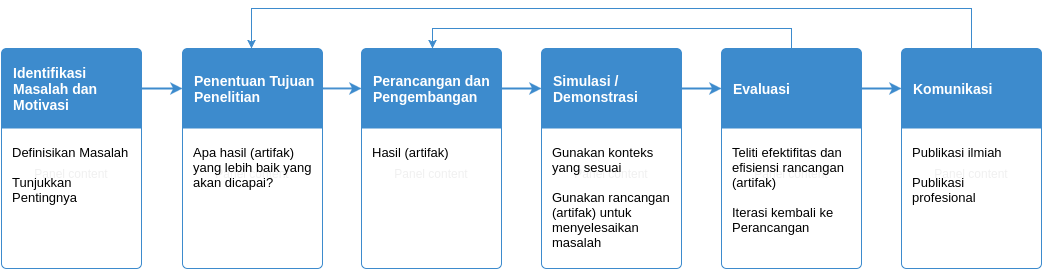
\includegraphics[width=13cm]{../../Resources/Images/dsrm}
    \caption{Tahapan \textit{Design Science Research Methodology (DSRM)}}
    \label{fig:dsrm}
\end{figure}

\begin{enumerate}
\item Identifikasi Masalah dan Motivasi


Langkah pertama dalam melakukan penelitian adalah dengan mengidentifikasi permasalahan sesungguhnya. Selain itu untuk melihat seberapa jauh pentingnya masalah tersebut terhadap sistem, hal ini dapat ditunjukkan pada dampak yang diperoleh apabila permasalahan tersebut tidak segera diatasi. Dengan mengetahui permasalahan, maka dapat diperoleh gambaran yang jelas terhadap masalah yang terjadi dan dapat menentukan batasan dari masalah tersebut. Tujuannya adalah untuk menentukan solusi seperti apa dan sejauhmana solusi tersebut sesuai dengan permasalahan yang terjadi.


\item Menentukan Tujuan dari Penelitian


Setelah melakukan identifikasi masalah, langkah selanjutnya yang dilakukan pada fase ini adalah mendefinisikan tujuan dari sebuah solusi berdasarkan identifikasi masalah dan informasi (knowledge) mengenai kondisi permasalahan yang telah dilakukan pada langkah sebelumnya. Tujuan dapat bersifat kuantitatif, misalnya, solusi yang diinginkan akan lebih baik daripada yang sekarang, atau kualitatif, misalnya, bagaimana metode baru ini diharapkan dapat mendukung solusi untuk masalah yang sampai sekarang belum bisa ditangani. Tujuan harus disimpulkan secara rasional dari spesifikasi masalah, kemampuan yang dibutuhkan untuk hal ini mencakup pengetahuan tentang keadaan masalah dan solusi yang akan dicapai.


\item Perancangan dan Pengembangan Solusi


Pelaksanaan tahap design and development pada DSRM adalah bertujuan untuk menghasilkan sebuah artefak baru yang bertujuan memberikan solusi terbaik dari problem yang dihadapi. Berikut beberapa jenis artefak yang dapat dihasilkan dari penerapan metode Design Science Research.


Dari Gambar ~\ref{fig:dsrm-artifact}, Purao membagi keluaran hasil penerapan DSRM menjadi tiga jenis alternatif model artefak, yaitu: munculnya sebuah model teori baru, atau sebuah metode pengembangan yang baru, atau juga dapat berupa instansiasi baru dari sebuah metode yang sudah ada ~\cite{purao_design_2002}.

\begin{figure}[h]
    \centering
    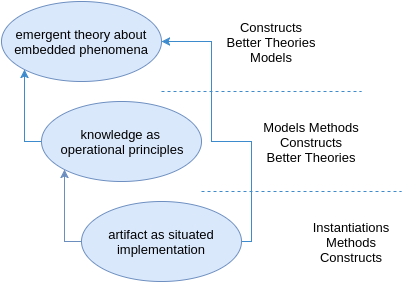
\includegraphics[width=7cm]{../../Resources/Images/dsrm-artifact}
    \caption{Artefak Hasil Penerapan Metode DSRM (Purao, 2002)}
    \label{fig:dsrm-artifact}
\end{figure}


\item Pembuatan Simulasi / Demonstrasi


Tahap demonstration bertujuan untuk menunjukkan cara penggunaan artefak (metode) baru untuk memecahkan satu atau lebih kasus dari masalah. Ini bisa melibatkan penggunaannya dalam eksperimen, simulasi, studi kasus, bukti, atau kegiatan lain yang sesuai. Kemampuan yang dibutuhkan untuk demonstrasi ini termasuk pengetahuan yang efektif tentang bagaimana menggunakan metode untuk memecahkan masalah.


\item Evaluasi


Tahap evaluasi dilakukan guna mengamati dan mengukur seberapa baik artefak (metode) baru mendukung solusi penyelesaian masalah. Kegiatan ini melibatkan pembandingkan tujuan solusi dengan hasil yang didapatkan terhadap penerapan metode baru yang dihasilkan. Hasil evaluasi yang didapat akan menjadi masukan bagi peneliti untuk memutuskan apakah penelitian akan beralih kembali ke langkah ketiga (design and development) untuk mencoba untuk meningkatkan efektivitas dari artefak atau untuk melanjutkan ke tahap keenam (communication) dan meninggalkan perbaikan lebih lanjut untuk proyek berikutnya.


\item Komunikasi


Tahap communication bertujuan untuk memberikan kesempatan kepada peneliti untuk menjelaskan tentang permasalahan yang diangkat dan pentingnya permasalahn itu untuk diteliti. Tahap ini juga berguna untuk menjelaskan bagaimana artefak baru berhasil dibuat, langkah-langkah yang dilakukan dalam menghasilkan artefak baru serta kelebihannya dalam memberikan solusi bagi permasalahan yang dihadapi. Communication dapat berupa dokumentasi publikasi penelitian ilmiah, peneliti mungkin menggunakan struktur penulisan karya tulis ilimiah dalam model communicationnya, seperti definisi masalah, tinjauan pustaka, pengembangan hipotesis, pengumpulan data, analisis, hasil, diskusi, dan kesimpulan.
\end{enumerate}


\section{Implementasi Metodologi}

Sebagaimana telah dijelaskan dalam bagian sebelumnya bahwa tahapan pelaksanaan riset terdiri dalam enam tahapan. Dalam pelaksanaannya, enam tahap dalam DSRM dibagi kedalam tiga aktivitas utama, yaitu: perancangan metode usulan, implementasi metode usulan, dan dokumentasi. Berikut tahapan pelaksanaan yang dilakukan dalam penelitian \theoriginaltitle.

\begin{figure}[h]
    \centering
    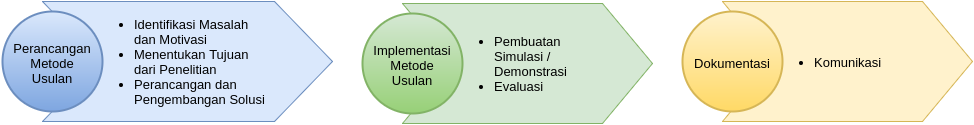
\includegraphics[width=1\textwidth]{../../Resources/Images/dsrm-implementation}
    \caption{Implementasi DSRM}
    \label{fig:dsrm-implementation}
\end{figure}


Perancangan metode usulan penelitian merupakan tahap awal yang dilakukan untuk menghasilkan sebuah metode baru. Tahap yang dilakukan pada fase perancangan metode usulan adalah : Identifikasi Masalah dan Motivasi, Menentukan Tujuan dari Penelitian, dan Perancangan dan Pengembangan Solusi. Implementasi metode usulan dilakukan dengan melakukan simulasi/uji coba metode usulan dalam kaitannya dengan pengumpulan data di BPS. Fase implementasi metode usulan terdiri dari : Pembuatan Simulasi / Demonstrasi dan Evaluasi. 

